\chapter{Event Reconstruction \& Simulation} \label{chap-EventReconstruction&Simulation}

Monte Carlo (MC) simulations are an essential part of current particle physics analyses and are used to mimic physical processes that correspond to those which are observed within the LHC, and other such experiments. Analysts compare to findings in data to simulation in order to extract signal processes, and also to perform statistical analysis on results obtained. It is of the utmost importance that the simulated events must be as accurate as physically possible in order to mimic real life processes and perform a scientifically accurate analysis. Will talk about methods for generating events, including the different MC generators and tunes used in the evaluation of theoretical uncertainties, and interpretation in terms of the CMS detector in the first section of this chapter.

Roughly speaking, we can divide the different steps of event reconstruction into three separate processes. The first of which records basic information, such as hits within the pixel detectors of the inner tracking system, and calorimeter energy clusters, for `low level' objects in each subdetector. The information is then passed to the PF algorithm which uses information from all the subdetectors in order to reconstruct events much more accurately. Finally, the events are refined by other complex statistic and mathematical techniques and used to reconstruct higher level objects, such as jets and MET. The second part of chapter will focus on the PF process \cite{CMS-PAS-PFT-09-001, CMS-PAS-PFT-10-001} as mentioned above.

Units \GeV sd

\section{Event Reconstruction} \label{sec-EventReconstruction}

\begin{figure} \label{fig-HadronCollisionProcess}
\begin{center}
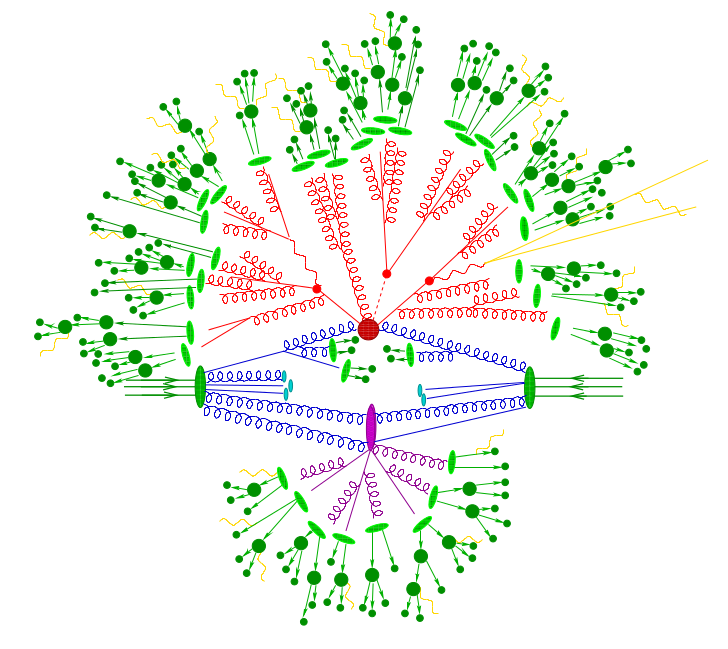
\includegraphics[scale=0.38]{Figures/HadronCollisionProcess.png}
\caption{Schematic overview of a hadron collision process \cite{HadronCollisionProcess}.}
\end{center}
\end{figure}

\section{Particle Reconstruction} \label{sec-ParticleReconstruction}

\subsection{Electron identification}

\subsection{Muon reconstruction}

\subsection{Jet reconstruction}

\subsubsection{Jet energy corrections}

\subsubsection{Particle flow jet identification}

\section{Computing}

\subsection{Event Data Model}

\subsection{Analysis Software}

\section{Monte Carlo Simulation}

\begin{sidewaystable} \label{tab-MCSamples}
\begin{center}
%\resizebox{\columnwidth}{!}

\begin{tabular}{|l| p{12.5cm} |c|p{2cm}|}
\hline
	\textbf{Process} & \textbf{Dataset} & \textbf{$\sigma$ (pb)} & \textbf{Number of events} \\
\hline
	$t\bar{t}+\gamma (2\to5)$ & /LHE2EDM\_WHIZARD\_2to5\_ttA/htholen-FULLSIM\_STEP2\_WHIZARD\_2to5\_ttA-da43ae45efb6a7c35e17aad82de2e2cd/USER & 1.8 & 1074860 \\
	$t\bar{t}+\gamma (2\to7)$ & /TTGamma\_TuneZ2star\_8TeV-madgraph-tauola/Summer12\_DR53X-PU\_RD1\_START53\_V7N-v1/AODSIM & 1.8 & 916500\\ 
\hline	
	$t\bar{t}(Leptonic)$ & /TTJets\_FullLeptMGDecays\_8TeV-madgraph/Summer12\_DR53X-PU\_S10\_START53\_V7A-v2/AODSIM & 245.8 & 12119013\\
	$t\bar{t}(Hadronic)$ & /TTJets\_HadronicMGDecays\_8TeV-madgraph/Summer12\_DR53X-PU\_S10\_START53\_V7A\_ext-v1/AODSIM & 245.8 & 31223821\\
	$t\bar{t}(Semileptonic)$ & /TTJets\_SemiLeptMGDecays\_8TeV-madgraph/Summer12\_DR53X-PU\_S10\_START53\_V7A\_ext-v1/AODSIM & 245.8 & 25424818\\
	$t\bar{t}(Inclusive)$ & /TTJets\_MassiveBinDECAY\_TuneZ2star\_8TeV-madgraph-tauola/Summer12\_DR53X-PU\_S10\_START53\_V7C-v1/AODSIM & 245.8 & 6923652\\
\hline	
	Drell-Yann, $10 < m\_{ll} < 50$ & /DYJetsToLL\_M-10To50\_TuneZ2Star\_8TeV-madgraph/Summer12\_DR53X-PU\_S10\_START53\_V7A-v1/AODSIM & 11050.0 & 37835275\\
	Drell-Yann, $m\_{ll} > 50$ & /DYJetsToLL\_M-50\_TuneZ2Star\_8TeV-madgraph-tarball/Summer12\_DR53X-PU\_S10\_START53\_V7A-v1/AODSIM & 3350.0 & 30459503\\
\hline	
	Single Top tW & /T\_tW-channel-DR\_TuneZ2star\_8TeV-powheg-tauola/Summer12\_DR53X-PU\_S10\_START53\_V7A-v1/AODSIM & 11.1 & 497658 \\
	Single TopBar tW $\bar{t}$ & /Tbar\_tW-channel-DR\_TuneZ2star\_8TeV-powheg-tauola/Summer12\_DR53X-PU\_S10\_START53\_V7A-v1/AODSIM & 11.1 & 493460 \\
	Single Top t & /T\_t-channel\_TuneZ2star\_8TeV-powheg-tauola/Summer12\_DR53X-PU\_S10\_START53\_V7A-v3/AODSIM & 56.4 & 99876 \\
	Single TopBar t & /Tbar\_t-channel\_TuneZ2star\_8TeV-powheg-tauola/Summer12\_DR53X-PU\_S10\_START53\_V7A-v1/AODSIM & 30.7 & 1935072 \\
	Single Top s & /T\_s-channel\_TuneZ2star\_8TeV-powheg-tauola/Summer12\_DR53X-PU\_S10\_START53\_V7A-v1/AODSIM & 3.79 & 259961 \\
	Single TopBar s & /Tbar\_s-channel\_TuneZ2star\_8TeV-powheg-tauola/Summer12\_DR53X-PU\_S10\_START53\_V7A-v1/AODSIM  & 1.76 & 139974 \\
\hline	
	W+Jets & /WJetsToLNu\_TuneZ2Star\_8TeV-madgraph-tarball/Summer12\_DR53X-PU\_S10\_START53\_V7A-v2/AODSIM & 36257.2 & 57709905\\
\hline	
	Diboson WW & /WW\_TuneZ2star\_8TeV\_pythia6\_tauola/Summer12\_DR53X-PU\_S10\_START53\_V7A-v1/AODSIM & 56.0 & 10000431\\
	Diboson WZ & /WZ\_TuneZ2star\_8TeV\_pythia6\_tauola/Summer12\_DR53X-PU\_S10\_START53\_V7A-v1/AODSIM & 33.6 & 10000283\\
	Diboson ZZ & /ZZ\_TuneZ2star\_8TeV\_pythia6\_tauola/Summer12\_DR53X-PU\_S10\_START53\_V7A-v1/AODSIM & 8.2 & 9799908\\
\hline	
\end{tabular}
\caption{Dataset information for signal and background MC samples.}
\end{center}
\end{sidewaystable}

\subsection{Monte Carlo event generators}



\begin{description}

	\item[\WHIZARD] \cite{WHIZARD} 

	\item[\MADGRAPH] \cite{MADGRAPH5} 

	\item[\PYTHIA] \cite{Sjöstrand2001238, 1126-6708-2006-05-026}

	\item[\MCATNLO] \cite{1126-6708-2002-06-029} 

	\item[\POWHEG] \cite{1126-6708-2007-11-070}

\end{description}	

\section{Simulation of the $t\bar{t}+\gamma$ Signal Sample} \label{subsec-mcsim}

Three different techniques were used to define the $t\bar{t}+\gamma$ signal process. The concepts are illustrated in Figure \ref{fig-MatrixElementCalculation} and shows the final state of the process using each technique \cite{heinerthesis}. The parton distribution function CTEQ6L1 \cite{Pumplin:2002vw} is interfaced to \WHIZARD via LHAPDF \cite{Whalley:2005nh}. The process utilises variable renormalisation and factorisation scales. This is such that, event by event, the two are set to $172.5 \GeV$ (m$_t$) plus the E$_T$ of the generated photon. Upon varying the scale of each, we arrive at a systematic uncertainty of $^{+7.0}_{-8.3}\%$, as shown in Chapter \ref{chap-SystematicUncertainties}.  Initial and final state radiation is taken into account, as well as hadronisation, and is simulated using PYTHIA6 [81], \TAUOLA and \PHOTOS (both in [82]) as preconfigured in CMSSW.

 The same configuration as for the top-pair sample is used, see Section 4.2.5.
FastSim is applied instead of the full detector simulation, automatically choosing a pileup
scenario that is tuned to 2011 data taking.

 Restrictions on the final state particles have been set, named generation cuts, such that a proper integral is retained when calculating matrix elements. As a method to cope with infra-red divergences, a minimum energy or momentum is required. We treat collinear divergences by introducing a minimum distance in the $\eta - \phi$ plane. These cuts likely will not affect the measurement due to the cuts within selection being tighter than generator levels cuts. The different generation cuts are described in brief below:

\begin{description}
\item[2 \to 3] At this level only quantum mechanical interferences from initial state radiation are considered. The CPU time required in for tree level processes is moderate.

\item[2 \to 5] In this case, the decay of the top quark is included and thus photons that have radiated from a W boson or a b-quark, as well as interference effects between the two, must be taken into account. This is a significant process, as we must expect photons stemming from a W or b to contribute significantly to our signal. Photons that are radiated from the W are considered negligible, because the W decay products are highly boosted in top-quark events giving rise to, mostly, collinear emissions. 

\item[2 \to 7] In this scenario we consider photon radiation and interference from all decay products. CPU time is much more intensive in this case due to the many more Feynman diagrams to be computed.                                                                            

\begin{figure}\label{fig-MatrixElementCalculation}
\begin{center}
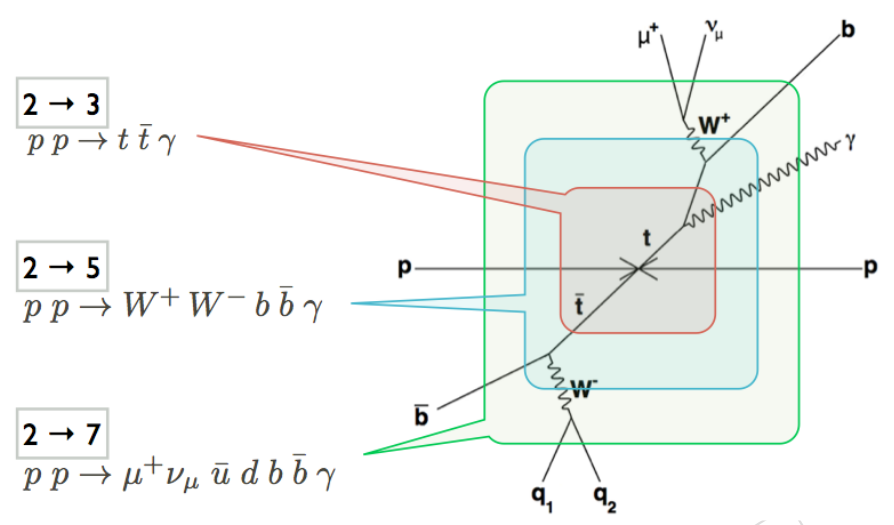
\includegraphics[width=\textwidth]{Figures/MatrixElementCalculation.png}
\caption{Process generation. The red, blue, and green boxes depict the matrix element calculation. Background processes with the same final state are included as well \cite{heinerthesis}.}
\end{center}
\end{figure}
                               

\end{description}

Originally, this analysis used the $2 \to 5$ technique with initial generator level cuts of $E_T > 20$ GeV and $\Delta R(\gamma, b/\bar{b}) > 0.1$ using WHIZARD \cite{WHIZARD}, which is a leading order (LO) event generator. The variable factorisation and renormalisation scales are set to $m_{top} + E_T(\gamma)$, and a scale variation uncertainty of 8\% has been applied to the WHIZARD $t\bar{t}+\gamma$ cross-section result, which gives $1.8 \pm 0.5$ pb as the SM expectation for the signal process, where the scale variation uncertainty, and uncertainty on the k-factor are added in quadrature. 


\subsection{Official $t\bar{t}+\gamma$ $2 \to 7$ process $\MADGRAPH$ Sample Production}

Details of signal sample generation are described in [7]. The phase space for generation was
chosen in the following way:

\begin{itemize}
	\item $p_T (\gamma) > 13 \GeV$
	\item $|\eta(\gamma)| < 3.0$
	\item $\Delta R (\gamma, all) > 0.3$, where `all' refers to any other generator level particle
	\item $p_T (jet) > 15 \GeV$
	\item $p_T (b) > 20 \GeV$
	\item $|\eta (b)| < 5.0$
	\item $|\eta (jet)| < 5.0$
	\item $| \eta (lepton)| < 3.0$
	\item $\Delta R (jet, jet) > 0.5$
	\item $\Delta R (jet, lepton) > 0.5$
\end{itemize}

There is no cut on lepton transverse momentum, but there are cuts on the momenta of quarks (jets). This makes the ratio of hadronic and leptonic W decays generated with these cuts differ from W branching ratio without any cuts.
